\documentclass[11pt,a4paper]{article}
\documentclass[11pt,a4paper]{article}
\usepackage[utf8]{inputenc}
\usepackage{amsmath}
\usepackage{amsthm}
\usepackage{amsfonts}
\usepackage{amssymb}
%\usepackage{algorithmic}
%\usepackage{algorithm}
\usepackage{hyperref}
%\usepackage[ruled,linesnumbered,procnumbered]{algorithm2e}

\makeatletter
\let\original@algocf@latexcaption\algocf@latexcaption
\long\def\algocf@latexcaption#1[#2]{%
  \@ifundefined{NR@gettitle}{%
    \def\@currentlabelname{#2}%
  }{%
    \NR@gettitle{#2}%
  }%
  \original@algocf@latexcaption{#1}[{#2}]%
}
\makeatother

\usepackage{xcolor}		% for adding colors to the text

\usepackage[footnotesize, center]{caption}	
\usepackage{subcaption}
%\usepackage{subfigure}
\usepackage{booktabs}
\usepackage{multirow}
\usepackage{breakurl}	% fixes the problem of breaking long url into lines inside the bibliography (IMP: must be below the hyperref package)
\hypersetup{
    bookmarks=true,		% show bookmarks bar?
    colorlinks=true,		% false: boxed links; true: colored links
    linkcolor=blue,		% color of internal links
    citecolor=blue,		% color of links to bibliography
    filecolor=blue,		% color of file links
    urlcolor=blue,		% color of external links
    bookmarksopen=true,
    breaklinks=true,
}
%\usepackage{natbib}			% bibliography
%\setlength{\bibsep}{0pt}

\usepackage[title]{appendix}

\usepackage{longtable}

% Page Setup

% Margins
	% MS Word (Default):		[margin=0.98in]
	% MS Word (Narrow):		[margin=0.5in]
\usepackage[margin=2cm]{geometry}
\setlength{\parskip}{\medskipamount}

\usepackage{setspace}
%\onehalfspacing
\setstretch{1.15}

\usepackage{indentfirst}			% indent the first paragraph
\allowdisplaybreaks				% break if equations take too much vertical space

% Section Style
\makeatletter
\def\@seccntformat#1{\csname the#1\endcsname.\quad}		% put a fullstop after section numbers
\makeatother

% Optional packages
\usepackage{xfrac}	% nicer fractional symbols (e.g., \sfrac{1}{2})
\usepackage{fancyhdr}	% adding headers / footers

% MACROS

% mathematical
\newcommand{\mathbold}[1]{\boldsymbol{#1}}		% for adding bold greek letters
\newcommand{\binary}{\{ 0, 1 \} }

\newcommand{\parentheses}[1]{\left( #1 \right) }	% auto-size parentheses
\newcommand{\brackets}[1]{\left[ #1 \right] }		% auto-size brackets
\newcommand{\curly}[1]{\left\{ #1 \right\} }		% auto-size curly brackets

	% Nilay Noyan's commenting macros
	% commentbox (adds black comments in a frame box)
	% comment (adds red comments as a footnote)

\newcounter{commentcounter}
\setcounter{commentcounter}{1}

\setlength{\fboxsep}{5pt}
\setlength{\fboxrule}{0.1pt}

\newcommand{\commentbox}[1]{
% \hfill \newline \noindent
%	\framebox[\textwidth]{
%		\parbox{0.98\textwidth}{
%			\footnotesize{
%				\texttt{\textcolor{black}{(C.\arabic{commentcounter})~#1\hfill}}}}}
%	\addtocounter{commentcounter}{1} 
	}

\long\def\symbolfootnote[#1]#2{\begingroup\def\thefootnote{\fnsymbol{footnote}}\footnote[#1]{#2}\endgroup}

\newcommand{\comment}[2]{{\footnotesize\texttt{\textcolor{red}{(C.\arabic{commentcounter})}}\symbolfootnote[4]{\texttt{\textcolor{red}
        {(C.\arabic{commentcounter}) [#1]: ~#2}}}}\addtocounter{commentcounter}{1}}
%\newcommand{\comment}[2]{}

% theorems
% the subtheorem environment is used to generate theorem numbers 1a, 1b, etc.
% Source: http://tex.stackexchange.com/questions/43346/how-do-i-get-sub-numbering-for-theorems-theorem-1-a-theorem-1-b-theorem-2
\makeatletter
\newenvironment{subtheorem}[1]{%
  \def\subtheoremcounter{#1}%
  \refstepcounter{#1}%
  \protected@edef\theparentnumber{\csname the#1\endcsname}%
  \setcounter{parentnumber}{\value{#1}}%
  \setcounter{#1}{0}%
  \expandafter\def\csname the#1\endcsname{\theparentnumber\alph{#1}}%
  \ignorespaces
}{%
  \setcounter{\subtheoremcounter}{\value{parentnumber}}%
  \ignorespacesafterend
}
\makeatother
\newcounter{parentnumber}
% end of subtheorem environment

\newtheorem{theorem}{\bf Theorem}
\newtheorem{lemma}{\bf Lemma}
\newtheorem{proposition}{\bf Proposition}
\newtheorem{corollary}{\bf Corollary}
\newtheorem{definition}{\sc Definition}
\newtheorem{fact}{\bf Fact}
\newtheorem{claim}{\sc Claim}
\newtheorem{case}{\sc Case}
\newtheorem{observation}{\sc Observation}
\renewcommand{\qedsymbol}{\hfill \tiny$\blacksquare$}		% symbol for proof environment
\renewcommand{\proofname}{\textnormal{\textbf{Proof.}}}	% title in the proof environment

\newtheoremstyle{mytheoremstyle} % name
    {\topsep}                    % Space above
    {\topsep}                    % Space below
    {}                   % Body font
    {}                           % Indent amount
    {\scshape}                   % Theorem head font
    {.}                          % Punctuation after theorem head
    {.5em}                       % Space after theorem head
    {}  % Theorem head spec (can be left empty, meaning ‘normal’)
\theoremstyle{mytheoremstyle}
\newtheorem{example}{Example}

\newtheoremstyle{myassumptionstyle} % name
    {\smallskipamount}                    % Space above
    {0}                    % Space below
    {}                   % Body font
    {}                     	% Indent amount
    {\upshape}              % Theorem head font
    {.}                          	% Punctuation after theorem head
    {.5em}                      % Space after theorem head
    {}  				% Theorem head spec (can be left empty, meaning ‘normal’)
\theoremstyle{myassumptionstyle}
\newtheorem{assumption}{\bf A\ignorespaces}
\newtheorem{remark}{\bf Remark}

\DeclareMathOperator*{\argmin}{arg\,min} 
\DeclareMathOperator*{\argmax}{arg\,max} 


% narrative
\newcommand{\ie}{\textit{i.e.}}		% id est, that is to say
\newcommand{\ex}{\textit{ex.}}		% example
\newcommand{\eg}{\textit{e.g.}}	% exempli gratia, for the sake of example

\newcommand{\st}{\text{subject to:}\qquad}	% subject to
\newcommand{\mathbi}[1]{\boldsymbol{#1}}	% \boldsymbol{ any character } // makes both italic and bold

\newcommand{\cplex}{\texttt{CPLEX}}

\newcommand{\question}[1]{\vspace{\baselineskip}\noindent\pdfbookmark{Question #1}{Question #1}\textbf{\large{Question #1}} \normalsize\medskip\newline}
\newcommand{\qpart}[1]{\indent\textbf{#1)}}	% i.e., a), b), ...

\newcommand{\inlinecomment}[1]{{\color[rgb]{0.13,0.57,0.4} \textbf{#1}}}

% algorithmic
\newcommand{\np}{$\mathcal{NP}$}	% e.g., as in NP-hard

\usepackage{enumitem}	% for aligned descriptions
\usepackage{calc} 		% for aligned descriptions

\setenumerate{
itemsep=0pt,
partopsep=0pt,
parsep=0pt,
topsep=0pt,
labelindent=4pt,
font=\normalfont
}

\setdescription{
itemsep=0pt,
partopsep=0pt,
parsep=0pt,
topsep=0pt,
labelindent=4pt,
font=\normalfont
}

\setitemize{
itemsep=0pt,
partopsep=0pt,
parsep=0pt,
topsep=0pt,
labelindent=4pt,
font=\normalfont
}


\usepackage{natbib}			% bibliography
\setlength{\bibsep}{0pt}

\setlength{\textheight}{23cm} %{23cm}
\setlength{\topmargin}{-2cm}
\setlength{\textwidth}{17.5cm} \setlength{\oddsidemargin}{-0.5cm}
\setlength{\evensidemargin}{-0.5cm}

\setlength{\parindent}{0pt}

\newcommand{\gap}{\vspace{5pt}}
\newcommand{\epc}{\hspace{1pc}}

\newcommand{\onebld}{{\bf 1}}
\newcommand{\wt}{\widetilde}
\newcommand{\wh}{\widehat}

\newcommand{\E}{{\rm I\!E}}
\newcommand{\IP}{{\rm I\!P}}
\newcommand{\D}{{\rm I\!D}}
\newcommand{\pmat}[1]{\begin{pmatrix} #1 \end{pmatrix}}
\newcommand{\us}[1]{{\color{black}#1}}
\newcommand{\ssbs}[1]{{\color{blue}#1}}
\bibliographystyle{apalike}

\title{\bf Taming the Duck: Can Stochastic Programming Help?}
\date{}
%\author{Harsha Gangammanavar\\Engineering Management, Information, and Systems\\Southern Methodist University, \\ Dallas, TX 75275}

\begin{document}
\pagenumbering{gobble}
\maketitle

\vspace*{-1.3cm}

\paragraph{Suvrajeet Theodore Sen:} 
The Quandary of Renewable Energy Integration

Lawmakers throughout the U.S. have mandated that electricity supply should include a significant percentage of energy from renewable resources - each state has set its own goal, with California being most aggressive requiring 50\% renewable energy by 2030.  Local/State authorities (e.g., Independent System Operators (ISO)) which are in-charge of wholesale electricity supply have commissioned focused studies to assess operational considerations such as system reliability, market design, storage technologies and other devices.  However a recent study commissioned by CAISO (see Olson et al 2015) suggest that for penetration levels beyond 33\%, there one can expect a great deal of over-generation  while also facing the possibility of curtailment of renewable energy, or load-shedding in the evening.  In case of curtailment of renewable energy, one faces the likelihood of negative prices in the market leading to large shipments of energy to neighboring states (e.g., Arizona) while paying those states to accept electricity from California. For the case of load-shedding, the loss of load probability (or loss of load expectation) can reach unacceptable levels, affecting system performance.  Page restrictions limit us from getting into more detailed discussions on the impact on GHG emissions due to the use of so-called fast-generators.  As these complications play out within the ISO communities, researchers in some environmental science programs have published a well-cited study in the Proceedings of the National Academy of Science (PNAS) where the authors suggest that renewable energy can be used to power 100\% of electricity requirements by 2050  (Jacobson et al 2017).  This study has come under heavy fire from a large group of engineers (Clack et al 2017) because the PNAS paper did not accommodate many engineering considerations such as transmission capacity, reliability and the like.   In addition to these considerations, the Federal Energy Regulatory Commission (FERC) has mandated that due to the volatility of renewable generators (solar and wind), electricity dispatch must take place at 10-15 minute intervals, instead of the usual hourly interval, which is the norm for fossil-fuel generators.  Such shorter dispatching intervals can help the system track changes in renewable generation.  However, these shorter time scales also calls for faster algorithms and faster computing environments.  In any event, it is important to recognize that just like any other infrastructure, reliability and efficient system operation requires us to strike a delicate balance between multiple facets such as generators, grids, natural resources, the weather, and of course market economics and public policy.  

The following is a small test grid example which is intended for academic tests of power system models. It is referred to as IEEE 118 (with 118 nodes/buses). Using the above network as a sample for experimenting with renewable energy, the National Renewable Energy Lab (NREL) has created a similar instance (called NREL 118) which represents a small grid (with 118 buses) and includes renewable resources together with conventional generators, and a transmission grid.  In addition, one can include market forces, weather models, and alternative renewable penetration policies to setup semi-realistic models which include statistical representations of wind, solar, and weather, economic representation of market equilibria, and operational models of resource utilization, reliability constraints and the like.  Such models have become an integral part of the OE community.  Our goal is to make realistic experimentation possible by allowing new models and algorithms for some aspects of the system, while leveraging the remaining data, models, and algorithms of a cyberinfrastructure which would be supplied within CORE.   A typical researcher who may  have an interest and expertise creating a new sub-model and/or algorithm, would be able to experiment with their new model/algorithm  by replacing the some of the functions of the CORE setup with their own trial  model/algorithm, while leveraging the remainder of the model/algorithm included within CORE.  In this way, the research community will be able to carry out experiments which test the approach within the broader context of the application.  Such experimentation will have the ability to establish benchmarks which are much more realistic than is available today. 

[1]	Clack, C.T.M. et al, 2017, “Evaluation of a proposal for reliable low cost grid power with wind, water, solar” Proceedings of the National Academy of Sciences, 114(26): 6722-6727.
[2]	Jacobson M. Z, et al. 2015, “100\% clean and renewable wind, water, and sunlightc(WWS) all-sector energy roadmaps for the 50 United States,”  Energy Environ Sci. 8:2093–2117.
[3]	Olson, A. et al 2015, “Halfway There:  Can California Achieve a 50\% Renewable Grid,” IEEE Power and Energy Magazine, 13(4): 41-93.


\paragraph{Harsha:} Renewable energy resources constitute a significant fraction of the nation's energy portfolio. It is expected that their contribution will increase at an astonishing $5\%$/year for the next $25$ years \cite{AEO2016}. A large portion of the forecasted renewable capacity addition will be provided by solar (from $25$ GW in 2015 to $246$ GW in 2040), followed by wind installations ($73$ GW between 2015 and 2040). While wind generation is hampered by the need to install new transmission lines to access remote wind sites, investments in solar generation has surged in recent years and it is expected to surpass wind capacity by 2032 \cite{AEO2016}. In any case, both these renewable resources exhibit three key characteristics: (a) variability - high magnitude changes in output in short duration of time, (b) uncertainty - unpredictable output, and (c) non-dispatchability - output limited to certain time periods in a day which does not coincide with demand. 

\gap{}

Variability and uncertainty of solar and wind generation pose significant technological and operational challenges, especially at high penetration levels. A particular difficulty arises due to frequent and large energy imbalances between total available resources and demand. These imbalances are addressed by system operators through procurement of additional operating reserves for short time frames (usually $5-60$ minutes). In our previous work \cite{Gang16a}, we have established that the amount of operating reserves necessary to maintain system reliability will increase with penetration of renewable resources. Serving half (as is the case in California \cite{SB350}) of the electric load with wind and solar requires an unprecedented level of these reserves. 

\gap

\begin{figure}
\centering
\vspace*{-0.6cm}
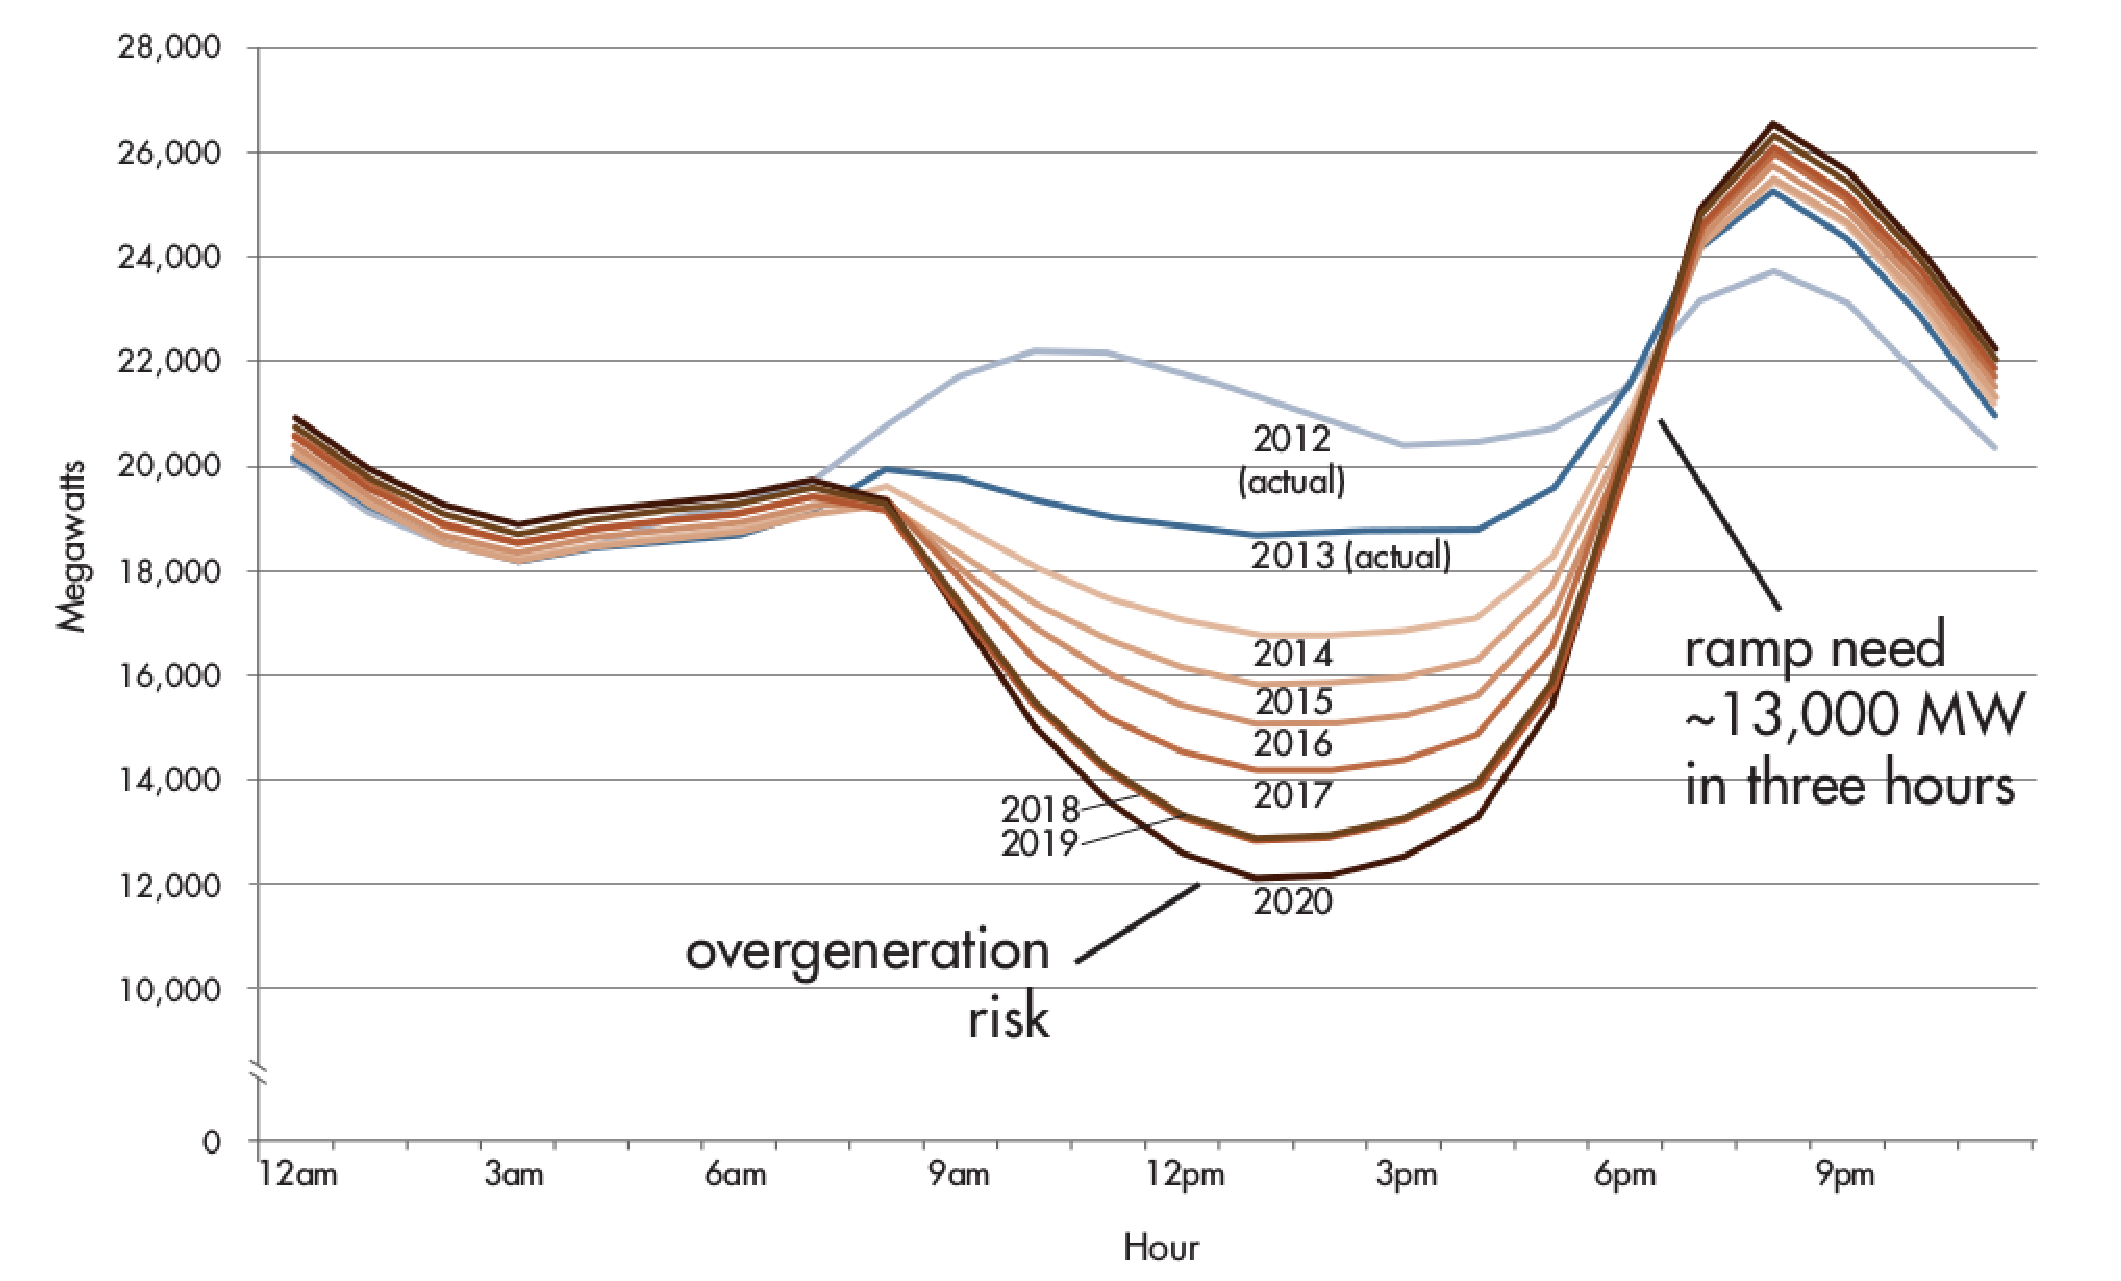
\includegraphics[scale=0.2]{./figures/duckChart}
\caption{CAISO's duck chart} \label{fig:duck}
\end{figure}

Non-dispatchability of wind and solar poses an even larger challenge for power system design. This is best illustrated in the widely circulated ``duck chart'' by California Independent System Operator (CAISO) which shows the net-load (difference between demand and generation) profile over successive years as more solar is installed \cite{Duck16}. The figure illustrates that the combination of increased load in the evening and reduction of solar generation at sundown creates a significant requirement for upward ramp. This may result in (1) an inability to meet the evening hour load due to insufficient upward ramping capability resulting in the undesirable load curtailment, (2) curtailment of renewable resources in the afternoon and allowing additional conventional generation to stay online, which reduces the effective capacity value of renewable resources and increases risk of over generation, and (3) procure sufficient upward ramping capability. The latter option has prompted CAISO and California Public Utilities Commission to propose ``flexible resource adequacy criteria and must offer obligations'' which requires California utilities to procure sufficient upward ramping capability \cite{FracMoo16}. These fast ramping reserves use fossil fuels (mainly, natural gas) and therefore undermine the original drive towards renewable resources, namely, reduction in CO2 emissions.

\gap

In light of these observations, our main questions are the following: (a) \textit{Is the power system reserve sufficient to support an ever-increasing renewable portfolio standards?}. We term a power system to be ``reserve sufficient'' if it has adequate reserves to maintain reliable operations at a certain renewable penetration level without undermining emission targets. (b) \textit{What is the impact of using advanced stochastic optimization tools for scheduling generators and operating reserves in power systems? Will it help achieve reserve sufficiency?} To achieve this we need:
\begin{enumerate} \itemsep0em
	\item {\it Develop reserve sufficiency models} which include different types of operating reserves, physical constraints of the power network, uncertainty in generation and demand, and differences in operating timescales of generators in the system. These models should capture the trade-off between an increase in renewable penetration and an increase in CO2 emissions from higher operating reserve utilization.
	\item {\it Develop an integrated stochastic optimization framework} which combines optimization and simulation. These stochastic frameworks should capture all the three characteristics of renewable generation and hence, offer an effective tool to establish reserve sufficiency.
\end{enumerate}

{\bf Design and Methodology}: Our framework uses suite of multiperiod stochastic programs that can be decomposed into a computationally viable form. Our preliminary model instances will be based on standard IEEE test systems \cite{Chri99}, which will then be scaled to a more realistic instance based on the Illinois power system used in \cite{Gang16a}. The uncertainty quantification related to renewable generation and demand will be based on open-access databases, such as WWSIS \cite{Pott08}. Our stochastic framework will use the stochastic mixed-integer Benders decomposition for commitment problems and two-stage stochastic decomposition \cite{Higl94} for economic dispatch as the optimization engines, and novel techniques to capture the hierarchical dynamics across time periods of operation. The focus will be on developing models that can be solved in a parallel/distributed environment high-performance computing resources. 
\newpage
{\bf Backdrop}: 
\begin{enumerate}
\item {\it ``Scheduling and Pricing for Expected Ramp Capability in Real-Time Power Markets''}: Variability is easier to accommodate than uncertainty. Since the changes are known, it can be scheduled for as long as the flexibility is available and resources are willing to provide it. It is possible that the capabilities of the supply mix are insufficient, and that even if the ramp required is known, the aggregate response speed is not capable of meeting it. When there is sufficient flexibility, the majority of expected variability that occurs on the system can usually be met explicitly through the previously discussed scheduling models. There are a few exceptions. First, it is possible that the variability is occurring at faster resolution than the scheduling model, and not enough information is available to meet this variability explicitly. Second, it is possible that the expected variability occurring in the future can affect the decisions that must be made now, and that information is beyond the scheduling horizon and not used within the scheduling model. 
\end{enumerate}

\newpage

{\bf Paragraphs: }

Lawmakers throughout the U.S. have mandated that electricity supply should include a significant percentage of energy from renewable resources --- each state has set its own goal, with California setting the most aggressive one as ``50\% renewable energy by 2030''.  

being the most aggressive and requiring 50\% renewable energy by 2030. Local / state authorities (e.g., Independent System Operators (ISOs)) which are in-charge of wholesale electricity supply have commissioned focused studies to assess operational considerations such as system reliability, market design, storage technologies and other devices.  However a recent study commissioned by CAISO (see Olson et al 2015) suggest that for penetration levels beyond 33\%, there one can expect a great deal of over-generation  while also facing the possibility of curtailment of renewable energy, or load-shedding in the evening.  In case of curtailment of renewable energy, one faces the likelihood of negative prices in the market leading to large shipments of energy to neighboring states (e.g., Arizona) while paying those states to accept electricity from California. For the case of load-shedding, the loss of load probability (or loss of load expectation) can reach unacceptable levels, affecting system performance.  Page restrictions limit us from getting into more detailed discussions on the impact on GHG emissions due to the use of so-called fast-generators.  As these complications play out within the ISO communities, researchers in some environmental science programs have published a well-cited study in the Proceedings of the National Academy of Science (PNAS) where the authors suggest that renewable energy can be used to power 100\% of electricity requirements by 2050  (Jacobson et al 2017).  This study has come under heavy fire from a large group of engineers (Clack et al 2017) because the PNAS paper did not accommodate many engineering considerations such as transmission capacity, reliability and the like.   In addition to these considerations, the Federal Energy Regulatory Commission (FERC) has mandated that due to the volatility of renewable generators (solar and wind), electricity dispatch must take place at 10-15 minute intervals, instead of the usual hourly interval, which is the norm for fossil-fuel generators.  Such shorter dispatching intervals can help the system track changes in renewable generation.  However, these shorter time scales also calls for faster algorithms and faster computing environments.  In any event, it is important to recognize that just like any other infrastructure, reliability and efficient system operation requires us to strike a delicate balance between multiple facets such as generators, grids, natural resources, the weather, and of course market economics and public policy.  

The following is a small test grid example which is intended for academic tests of power system models. It is referred to as IEEE 118 (with 118 nodes/buses). Using the above network as a sample for experimenting with renewable energy, the National Renewable Energy Lab (NREL) has created a similar instance (called NREL 118) which represents a small grid (with 118 buses) and includes renewable resources together with conventional generators, and a transmission grid.  In addition, one can include market forces, weather models, and alternative renewable penetration policies to setup semi-realistic models which include statistical representations of wind, solar, and weather, economic representation of market equilibria, and operational models of resource utilization, reliability constraints and the like.  Such models have become an integral part of the OE community.  Our goal is to make realistic experimentation possible by allowing new models and algorithms for some aspects of the system, while leveraging the remaining data, models, and algorithms of a cyberinfrastructure which would be supplied within CORE.   A typical researcher who may  have an interest and expertise creating a new sub-model and/or algorithm, would be able to experiment with their new model/algorithm  by replacing the some of the functions of the CORE setup with their own trial  model/algorithm, while leveraging the remainder of the model/algorithm included within CORE.  In this way, the research community will be able to carry out experiments which test the approach within the broader context of the application.  Such experimentation will have the ability to establish benchmarks which are much more realistic than is available today. 

\paragraph{Basics of Power-Systems Operations}
Power-systems are typically managed in two-phases. The first phase involves \emph{day-ahead} planning, where demand and renewable-supplies are estimated, generation-bids are collected, and a day-ahead unit-commitment (DAUC) problem is solved to clear the market. The DAUC problem produces a low-cost commitment-schedule for all generating units, over a day-long planning-horizon with one-hour resolution. Additional capacities, such as operating reserves, are also procured in the day-ahead market \citep{Doherty2005, Morales2009}. The second-phase of operations addresses the \emph{real-time} requirements of the grid. Throughout the day, economic-dispatch (ED) problems are periodically solved to determine the generation-schedules of committed units. These problems are typically solved for a much shorter time-horizon but with finer resolution. Additional needs, such as precautionary reliability measures, are also assessed and addressed during real-time operations. 

\paragraph{ISO Practices} In practice, ISO operations may significantly vary across different authorities, and can get much more complex. For instance, Bonneville Power Administration, which primarily produces hydro-electricity, performs bulk-hourly generation-scheduling, and has sufficient range of load-following, regulation, and ramping capabilities for handling within-hour imbalances \citep{Makarov2010}. Advanced ISOs, such as New York ISO, consider additional UC problems with finer resolution, in order to make adaptive (de)commitment decisions in real-time \citep{NYISO2017}. The California ISO, an authority that is under stress due to the state's ambitious renewable goals, makes use of a multitude of UC and ED problems, both for day-ahead planning and real-time operations. Each of these problems serve a different purpose, may be solved periodically throughout the day, and may have resolutions as low as 5 minutes \citep{CAISO2017}. The level of sophistication, among other things, allows the use of up-to-date renewable-supply estimations in real-time, and helps maintaining the reliability and cost-effectiveness of the grid.

\paragraph{Neglecting Uncertainty} Modern ISOs rely on sophisticated prediction models to make accurate load and renewable-supply predictions \citep[see, for instance,][]{CAISO2017, NYISO2017}. These models produce a single \textit{expected} time-series, which is, then, fed into optimization models, for the commitment- and generation-schedules to be determined. Ordinarily, these optimization models are \textit{deterministic} in nature, therefore assume that the expected time-series is the only possible realization of the future. Accordingly, produced decisions may only be \textit{optimal} with respect to this expected time-series, and potentially disregard the uncertainty of estimation-errors. For systems where uncertainty is a big factor, the optimization literature has well-documented that deterministic-natured decisions, indeed, demonstrate poor performance in simulation studies \citep[see, for a study on energy-systems,][]{Gangammanavar2016}.

\comment{SA}{Talk about stochastic optimization models now.}

%\begin{itemize}
%    \item ISOs have sophisticated models to make accurate load and renewable-supply predictions. 
%    \item However, this only accounts for the variability of these stochastic processes, whereas uncertainty is left untreated in the optimization models.
%    \item Demand Forecasts are obtained through neural-network- and regression-based methodologies, which are published, in advance, for the day-ahead market, and at the real-time \cite{CAISO2017, NYISO2017}.
%\end{itemize}

\texttt{What are we doing and why?}

In the first part of our study, we demonstrate the increased renewable-integration can cause stress in the grids

\cite{Olson2015}

Then, in the second part, we will introduce certain algorithmic novelties to the decision process. This will illustrate, how much we can go forward, without physical inventions, etc. 

\paragraph{Experimental Framework for Approximating ISO Operations}
We adopt a three-layered hierarchical framework to approximate realistic power-systems operations. At first, a DAUC problem is solved to determine hourly commitment-schedules for the majority of generating units.
% The DAUC problem uses the best-available load and renewable-supply forecasts in day-ahead.
Then, in real-time, we consider a short-term UC (STUC) problem to be solved every hour. This problem produces commitment-decisions for the remaining (fast-start) generators, and generation-decisions for all generating units, over a 3-hour time horizon with 15-minute resolution. The STUC problem gives the grid the necessary flexibility to accommodate sudden drops in actual or forecasted renewable-supply amounts. Finally, every 15 minutes, we solve an ED problem to determine real-time dispatch amounts over a 1-hour time horizon with 15-minute resolution. The timeline of our framework is illustrated in Figure \ref{fig:framework}.

\paragraph{Incorporating Optimization-under-Uncertainty into ISO Operations}

\newpage

\textbf{Further reading: }

\paragraph{CAISO - BPM Market:}

\texttt{[pg 155]} Overgeneration condition in IFM may manifest when self-scheduled supply exceeds total bid-in demand. In this case, overgeneration will be resolved by reducing self-scheduled generation through the adjustment of non-priced quantities pursuant to the scheduling priorities specified in Section 31.4.

If the scheduled CAISO Demand exceeds the CAISO Forecast of CAISO Demand when performing RUC, RUC may reduce supply scheduled in IFM down to minimum load through uneconomic adjustments but RUC does not automatically de- commit a resource scheduled in IFM. The CAISO Operator may communicate the need for de- commitment of resources with affected Market Participants.

If the Overgeneration condition continues in Real-Time, RTM attempts to dispatch resources down using economic Bids to the extent possible to relieve the Overgeneration condition. If use of economic Bids is insufficient, then supply curtailment is performed through uneconomic adjustments in the order established in accordance with Section 34.10.2 of the CAISO Tariff. Additionally, RTUC may optimally de-commit resources in real time (refer to section 7). Lastly, Exceptional Dispatches may be necessary to resolve the Overgeneration condition including situations created by “virtual” overgeneration in the IFM due to Virtual Bidding. Exceptional Dispatches may also include manual resource de-commitment.

\texttt{[pg 198]} As described above, the IFM clears the market based on the Self-Schedules and Economic Demand Bids of the SCs, and as a result it may clear at an overall level that is significantly lower than the CAISO Forecast of CAISO Demand for the next day. The purpose of the RUC process is to assess the resulting gap between the IFM Scheduled Load and the CAISO Forecast of CAISO Demand, and to ensure that sufficient capacity is committed or otherwise be available for Dispatch in Real-Time in order to meet the Demand Forecast for each Trading Hour of the Trading Day.

\texttt{[pg 200]} The objective of the RUC optimization is to minimize the incremental Start-Up, Minimum Load and incremental RUC Availability Bids in order to ensure sufficient resources are committed and/or capacity is available to meet the adjusted CFCD for each hour over 24 hours of the next Operating Day,

\url{http://www.caiso.com/market/Pages/MarketProcesses.aspx}

Day-ahead market
The day-ahead market is made up of three market processes that run sequentially. First, the ISO runs a market power mitigation test. Bids that fail the test are revised to predetermined limits. Then the integrated forward market establishes the generation needed to meet forecast demand. And last, the residual unit commitment process designates additional power plants that will be needed for the next day and must be ready to generate electricity. Market prices set are based on bids.

A major component of the market is the full network model, which analyzes the active transmission and generation resources to find the least cost energy to serve demand. The model produces prices that show the cost of producing and delivering energy from individual nodes, or locations on the grid where transmission lines and generation interconnect.

Scheduling coordinators (SCs) are pre-qualified entities authorized to transact in the ISO market. The day-ahead market opens for bids and schedules seven days before and closes the day prior to the trade date. Results are published at 1:00 p.m.

Real-time market
The real-time market is a spot market in which utilities can buy power to meet the last few increments of demand not covered in their day ahead schedules. It is also the market that secures energy reserves, held ready and available for ISO use if needed, and the energy needed to regulate transmission line stability.

The market opens at 1:00 p.m. prior to the trading day and closes 75 minutes before the start of the trading hour. The results are published about 45 minutes prior to the start of the trading hour. The real-time market system dispatches power plants every 15 and 5 minutes, although under certain grid conditions the ISO can dispatch for a single 1-minute interval.

Real-Time Unit Commitment (RTUC) is a market process for committing Fast and Short-Start Units and awarding additional AS from Dynamic System Resources at 15-minute intervals. The RTUC function runs every 15 minutes and looks ahead in 15-minute intervals spanning the current Trading Hour and next Trading Hour. Refer to Section 7.6, Real-Time Unit Commitment. Also refer to Exhibit 6-2, Generating Unit Commitment Selection by Application, for a summary of the Unit Commitment processes.
The Fifteen Minute Market (FMM) is the second interval of the RTUC and its results produce the binding FMM

Short-Term Unit Commitment (STUC) is a reliability function for committing Short and Medium Start Units to meet the CAISO Forecast of CAISO Demand. The STUC function is performed hourly and looks ahead three hours beyond the Trading Hour, at 15-minute intervals. Refer to Section 7.7, Short-Term Unit Commitment.

2.3.2.5 Real-Time Economic Dispatch
The Real-Time Economic Dispatch (RTED) is a market process that dispatches Imbalance Energy and dispatches Energy from AS and normally runs automatically every five minutes to
produce Dispatch Instructions. The following two alternative modes to RTED are invoked under abnormal conditions:

- Real-Time Contingency Dispatch (RTCD)

- Real-Time Manual Dispatch (RTMD)

Refer to Section 7.8, Real-Time Economic Dispatch, and Attachment A.2, Security Constrained Economic Dispatch, for a description of the Dispatch algorithm.

2.3.2.5.1 Real-Time Contingency Dispatch
The Real-Time Contingency Dispatch (RTCD) function executes upon CAISO Operator action, usually following a Generating Unit or transmission system Contingency. The RTCD execution is for a single 10-minute interval and includes all Operating Reserves and all Real-Time Energy Bids in the optimization process. Refer to Section 7.9, Real-Time Contingency Dispatch.
2.3.2.5.2 Real-Time Manual Dispatch
The Real-Time Manual Dispatch (RTMD) function executes upon CAISO Operator action, usually when RTED and RTCD fail to provide a feasible solution. The RTMD is manually executed every five minutes for a single 5-minute interval. Refer to Section 7.10, Real-Time Manual Dispatch.


\textbf{NYISO}

Day-Ahead Scheduling Subsystem
The Day-Ahead scheduling process consists of the following principal functions:

- Assemble Day-Ahead Transmission Outages; Update Total Transfer Capabilities, constraints and the Security Constrained Unit Commitment (SCUC) model; post updated Total Transmission Capability on the Open Access Same Time Information System.

- Produce NYISO Day-Ahead Zonal Load Forecast, based on weather forecasts and the load forecast model.

- Perform SCUC and scheduling.

- Tabulate and Evaluate Non-Firm Transactions; In the event that there is no congestion, the non-firm transactions are scheduled in sequence up to the Available Transfer Capabilities of the NYS Transmission System.

- Perform Automated Mitigation of generator offers.

Real-Time Scheduling Subsystem
Approximately every 15 minutes, a Real-Time Commitment (RTC) evaluation takes place to ensure that the schedules meet all of the reliability requirements. Each Real-Time transaction is evaluated independently against the Day-Ahead transactions and Generator Bids, using the RTC program. Any new firm External Transactions will be scheduled by RTC, which could displace some of the Day-Ahead non-firm transactions. If necessary, 10 and 30-minute resources will also be scheduled. The results are then posted every 15 minutes.
Approximately every 5 minutes, the Real-Time Dispatch (RTD) uses Bid curves of the New York Control Area (NYCA) generators to dispatch the system to meet the load while observing transmission constraints. Bid curves will consist of a combination of incremental bid curves provided by generators bidding into the LBMP market and decremental bid curves provided by generators serving Bilateral Transactions.

There is no such thing as a “Must Run” generator. To improve the chances that a generator is scheduled into the market, it must be offered such that it is positioned at the bottom of the economic bid curve.

\bibliography{references}

% \begin{thebibliography}{9}

% \bibitem{AEO2016}
%     \emph{``Annual Energy Outlook''}, 2016, U.S. Energy Information Administration, DOE/EIA-0383.

% \bibitem{Gang16a}
% 	H. Gangammanavar, S. Sen and V. M. Zavala, \emph{``Stochastic Optimization of Sub-Hourly Economic Dispatch With Wind Energy,''} in IEEE Transactions on Power Systems, vol. 31, no. 2, pp. 949-959, March 2016.

% \bibitem{Gang16b} H. Gangammanavar and S. Sen, \emph{``Two-scale Stochastic Optimization for Controlling
% Distributed Storage Devices,''} accepted for publication in IEEE Transactions on Smart Grid, 2016.

% \bibitem{SB350}  California Legislative Information, \emph{``SB-350 Clean Energy and Pollution Reduction Act of 2015''} , Sacramento, CA, October 7, 2015.

% \bibitem{Duck16} \emph{``California ISO - Fast Facts''} available at \href{https://www.caiso.com/Documents/FlexibleResourcesHelpRenewables_FastFacts.pdf}{https://www.caiso.com}.

% \bibitem{FracMoo16} \emph{``Flexible resource adequacy criteria and must offer obligations''}, available at \href{https://www.caiso.com/informed/Pages/StakeholderProcesses/FlexibleResourceAdequacyCriteria-MustOfferObligations.aspx} {https://www.caiso.com}.
% %\bibitem{FracMoo16} \emph{``Flexible resource adequacy criteria and must offer obligations''}, available at \href{https://www.caiso.com/informed/Pages/StakeholderProcesses/FlexibleResourceAdequacyCriteria-MustOfferObligations.aspx} {https://www.caiso.com}.

% \bibitem{Chri99} R. D. Christie, \emph{``Power Systems Test Case Archive''}, available at \href{http://www.ee.washington.edu/research/pstca/} {http://www.ee.washington.edu/research/pstca/}, 1999.

% \bibitem{Pott08} C. W. Potter, et al., \emph{``Creating the Dataset for the Western Wind and Solar Integration Study ({U}.{S}.{A}.)''}, Wind Engineering, vol. 32, no. 4, pp. 325-338, 2008.

% \bibitem{Higl94} J.L. Higle, and S. Sen, \emph{``Finite master programs in regularized stochastic decomposition''}, Mathematical Programming, vol. 67, pp. 143-168, 1994.

% \bibitem{Olso15} A. Olson et al., \emph{``Halfway There: Can California Achieve a 50\% Renewable Grid?},'' in IEEE Power and Energy Magazine, vol. 13, no. 4, pp. 41-52, July-Aug. 2015.

% \end{thebibliography}

\end{document}
